\documentclass[final]{beamer}
% http://tex.stackexchange.com/questions/56205/wrapfigure-beamer-style
\usepackage{color}
%\usepackage{cutwin}
%\usetheme{RJH}
\usetheme{Berkeley}
%\usetheme{Bergen}
\usepackage[orientation=portrait,size=a0,scale=1.4,debug]{beamerposter}
\usepackage[absolute,overlay]{textpos}
\setlength{\TPHorizModule}{1cm}
\setlength{\TPVertModule}{1cm}

% RGB (145,201,219), #91C9DB
%\definecolor{mybluelabel}{RGB}{145,201,219}
% RGB (48,174,228), #30AEE4
\definecolor{mybluelabel}{RGB}{48,174,228}

%\title{Data-Intensive Analysis for High Energy Physics (DIANA/HEP)}
%\author{Peter Elmer}
%\date{}

\begin{document}
\begin{frame}{} 

\begin{textblock}{20}(2,2)
\begin{center}
\begin{figure}[tbph]
\centering
%
\includegraphics[width=0.45\textwidth]{images/dianahep-logo.png}

\includegraphics[width=0.70\textwidth]{images/diana-hep-06-logo-horizontal.png}
\end{figure}
\url{http://diana-hep.org}
\end{center}
\end{textblock}


\begin{textblock}{84.0}(6,2)
\begin{center}
\begin{LARGE}
Data-Intensive Analysis for High Energy Physics (DIANA/HEP)
\end{LARGE}
\end{center}
\end{textblock}

\begin{textblock}{84.0}(6,5)
\begin{center}
\begin{Large}
PIs: Peter Elmer (Princeton U.), Brian Bockelman (U.Nebraska-Lincoln), \\ 
Kyle Cranmer (NYU), Mike Sokoloff (U.Cincinnati)
\end{Large}
\end{center}
\end{textblock}

\begin{textblock}{38.0}(4,10)
\begin{block}{High Energy Physics (HEP)}
%\begin{center}
The quest to understand the fundamental building blocks of nature,
and their interactions, is one of the longest running and most
ambitious of human endeavors. Facilities such as the Large Hadron
Collider (LHC), where we do our research, represent a huge step
forward in our ability to answer these questions. The discovery of
the Higgs boson, the observation of exceedingly rare decays of B
mesons, and exclusion of countless theories beyond the Standard
Model (SM) of particle physics demonstrate that these experiments
deliver results. However, the most interesting fundamental physics
questions remain wide open, amongst them: What is the dark matter
which pervades the universe? Does space-time have additional
symmetries or extend beyond the 3 spatial dimensions we know? What
is the mechanism stabilizing the Higgs mass from enormous quantum
corrections? Are neutrinos, whose only SM interactions are weak,
their own anti-particles? Can the theories of gravity and quantum
mechanics be reconciled? Planned and running HEP experiments 
aim to answer these questions over the next 20 years.
~~~ \\
~~~ \\
\begin{figure}[tbph]
\centering
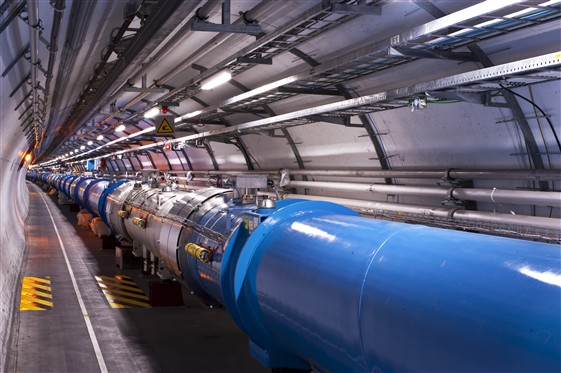
\includegraphics[width=0.48\textwidth]{images/0910152_02-A5-at-72-dpi.jpg}
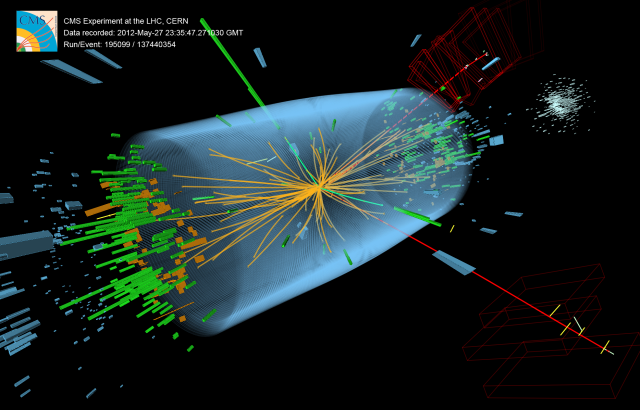
\includegraphics[width=0.50\textwidth]{images/eemm_run195099_evt137440354_ispy_3d-annotated-2.png}
\begin{center}
{\small \copyright~2009-2016 CERN (License: CC-BY-SA-4.0)}
\end{center}
\end{figure}
\end{block}
\end{textblock}

%\begin{textblock}{38.0}(44,10)
%\begin{block}{~~}
%\begin{figure}[tbph]
%\centering
%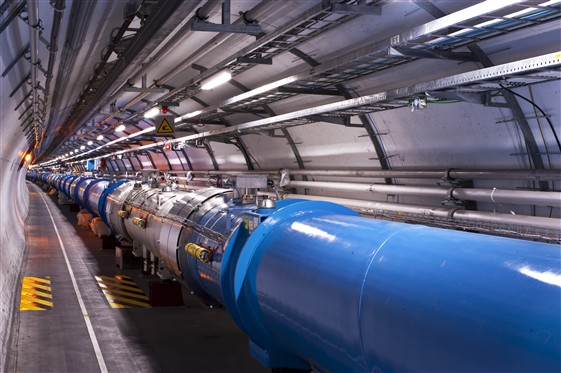
\includegraphics[width=0.48\textwidth]{images/0910152_02-A5-at-72-dpi.jpg}
%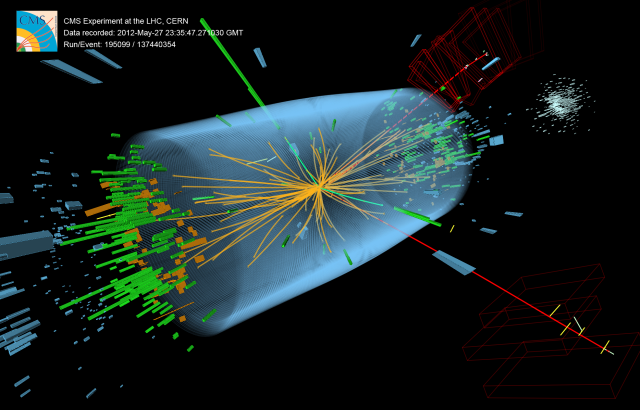
\includegraphics[width=0.50\textwidth]{images/eemm_run195099_evt137440354_ispy_3d-annotated-2.png}
%\begin{center}
%{\small \copyright~2009-2016 CERN (License: CC-BY-SA-4.0)}
%\end{center}
%\end{figure}
%\end{block}
%\end{textblock}



%\begin{textblock}{38.0}(4,10)
\begin{textblock}{38.0}(44,10)
\begin{block}{The DIANA/HEP Project}
The primary goal of DIANA/HEP is to develop state-of-the-art tools
for experiments which acquire, reduce, and analyze petabytes of
data. Improving performance, interoperability, and collaborative
tools through modifications and additions to ROOT and other packages
broadly used by the community will allow users to more fully exploit
the data being acquired at CERN's Large Hadron Collider (LHC) and
other facilities. The LHC experiments, for example, use nearly 0.5 Exabyte of
storage today, and planned upgrades through the 2020s will increase this
by more than a factor of 100. 
%\begin{figure}[tbph]
%\centering
%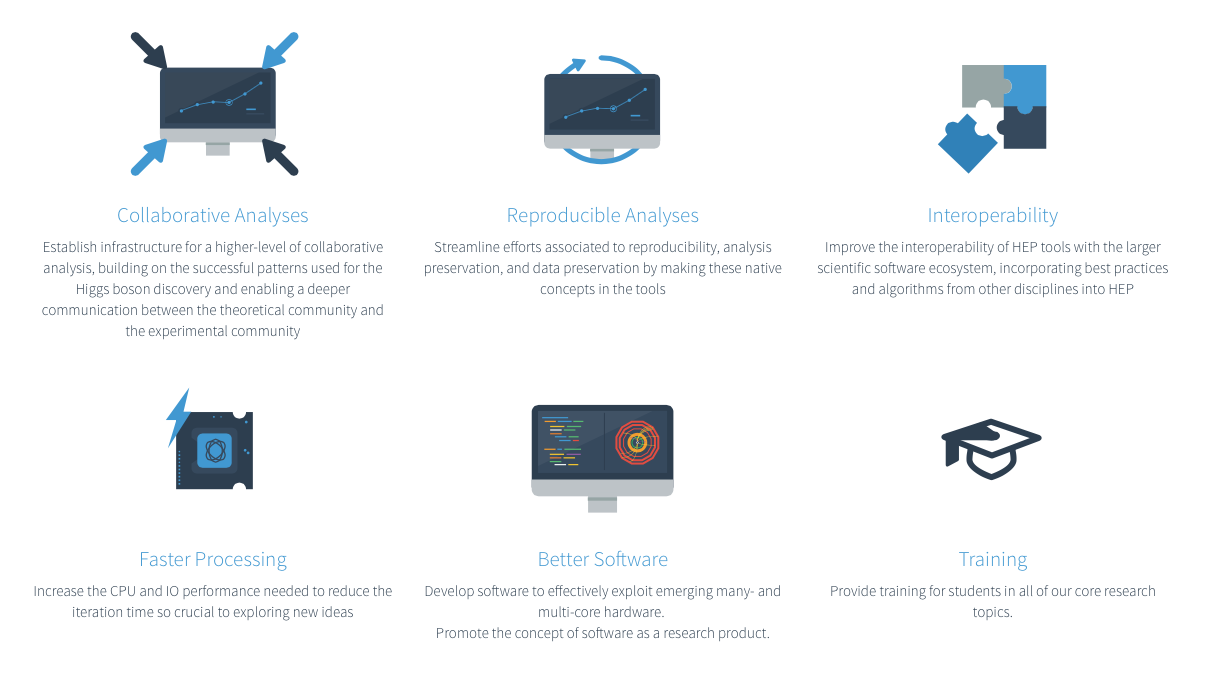
\includegraphics[width=0.8\textwidth]{images/diana-hep-goals.png}
%\end{figure}
\end{block}
\end{textblock}

\begin{textblock}{78.0}(4,52)
\begin{block}{Project Goals}
\end{block}
\end{textblock}

\begin{textblock}{22.5}(4,55.5)
\textcolor{mybluelabel}{\bf Collaborative Analyses} \\
Establish infrastructure for a higher-level of collaborative analysis, building on the successful patterns used for the Higgs boson discovery and enabling a deeper communication between the theoretical community and the experimental community. 
\end{textblock}

\begin{textblock}{12.5}(27.5,55)
\begin{figure}[tbph]
\centering
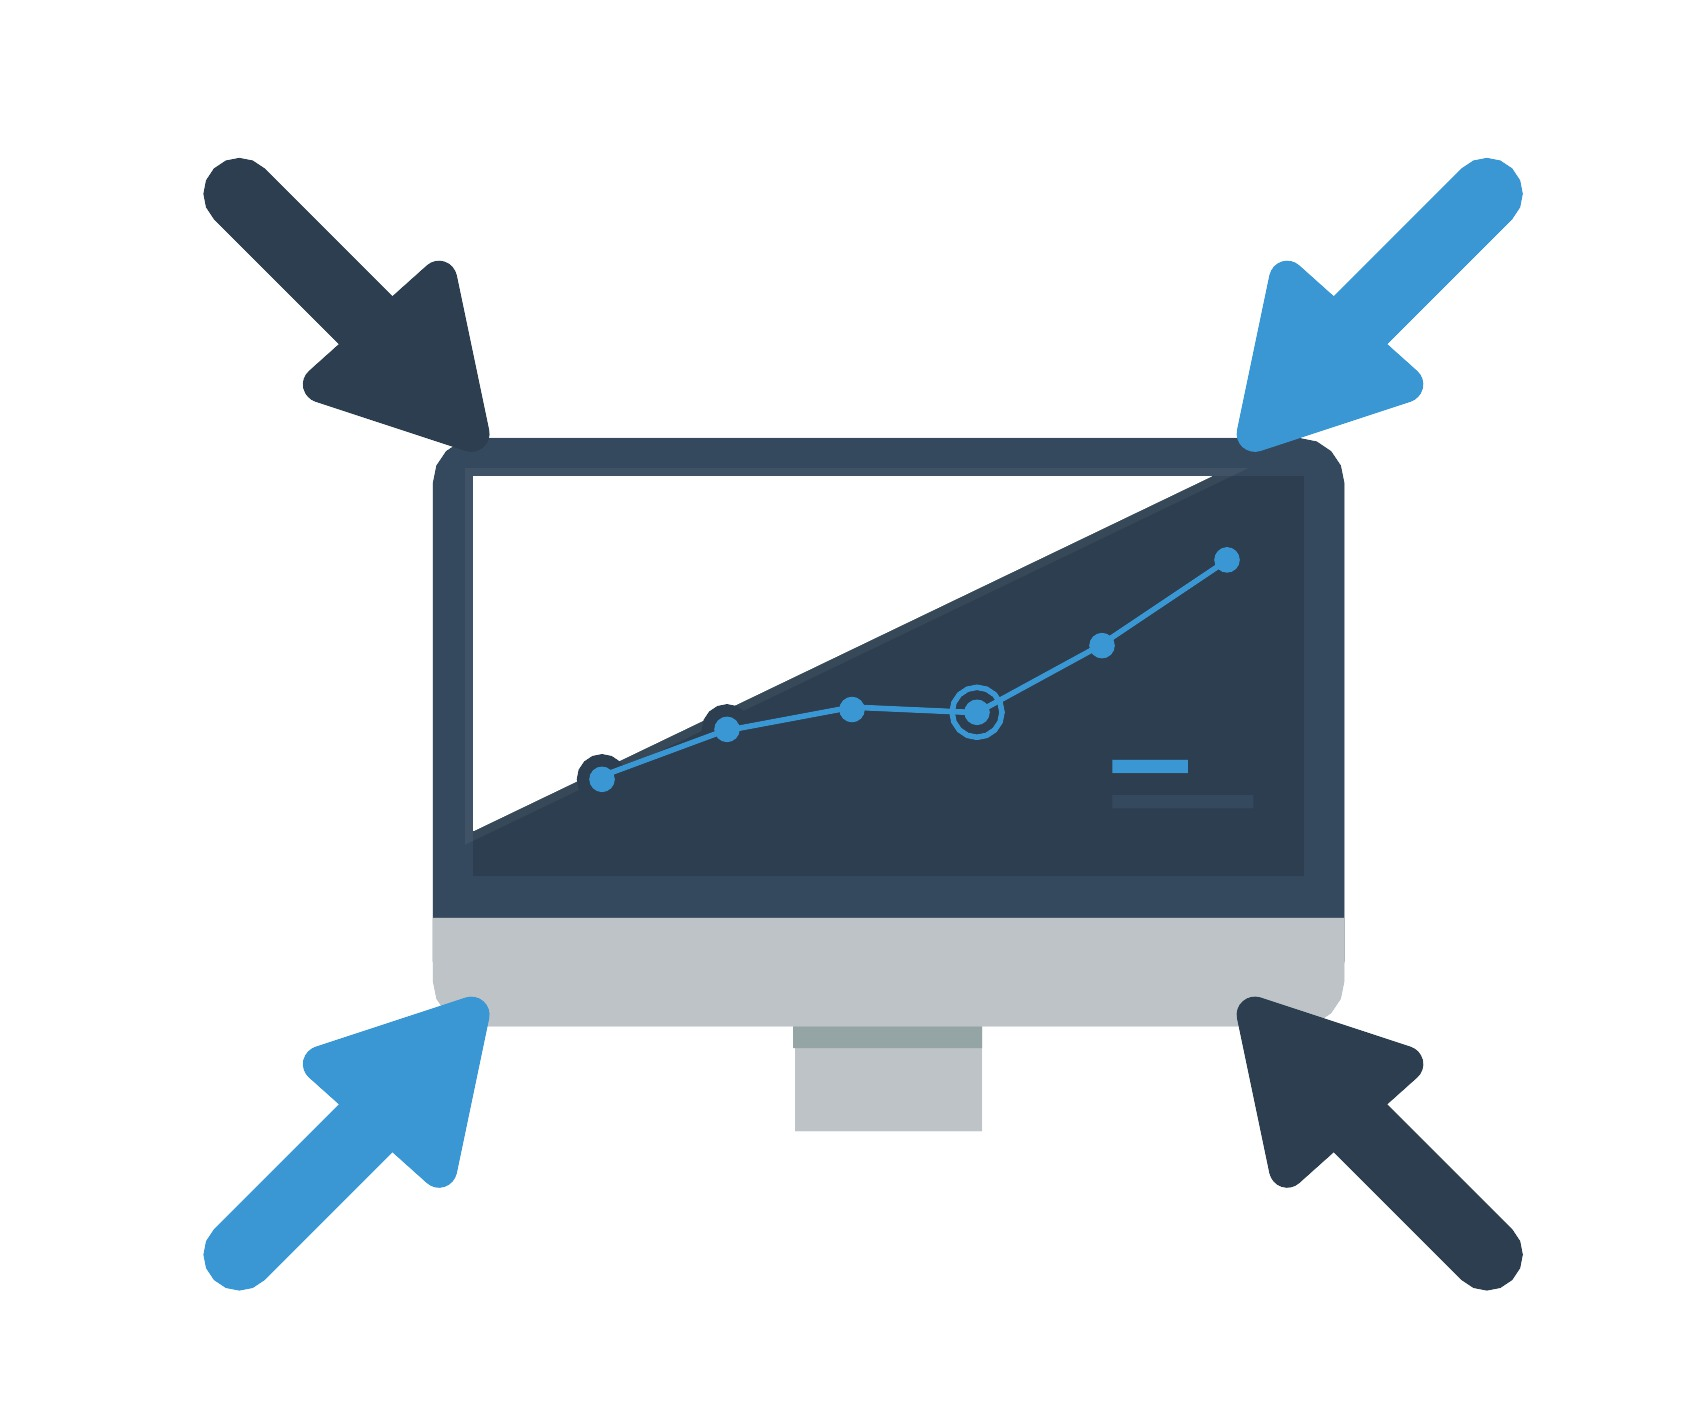
\includegraphics[width=0.8\textwidth]{images/collaborate.jpg}
\end{figure}
\end{textblock}

%%%

\begin{textblock}{22.5}(4,68)
\textcolor{mybluelabel}{\bf Faster Processing} \\
Increase the CPU and IO performance needed to reduce the iteration time so crucial to exploring new ideas
\end{textblock}

\begin{textblock}{12.5}(27.5,68)
\begin{figure}[tbph]
\centering

\includegraphics[width=0.6\textwidth]{images/faster-processing.jpg}
\end{figure}
\end{textblock}

%%%

\begin{textblock}{22.5}(4,77)
\textcolor{mybluelabel}{\bf Reproducible Analyses} \\
Streamline efforts associated to reproducibility, analysis preservation, and data preservation by making these native concepts in the tools.
\end{textblock}

\begin{textblock}{12.5}(27.5,77)
\begin{figure}[tbph]
\centering
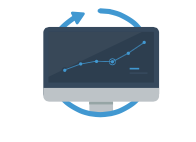
\includegraphics[width=0.8\textwidth]{images/reproducible-ss.png}
\end{figure}
\end{textblock}

%%%

\begin{textblock}{22.5}(44,55.5)
\textcolor{mybluelabel}{\bf Interoperability} \\
Improve the interoperability of HEP tools with the larger scientific software ecosystem, incorporating best practices and algorithms from other disciplines into HEP.
\end{textblock}

\begin{textblock}{12.5}(67.5,55)
\begin{figure}[tbph]
\centering

\includegraphics[width=0.8\textwidth]{images/interoperable.jpg}
\end{figure}
\end{textblock}

\begin{textblock}{23}(44,68)
\textcolor{mybluelabel}{\bf Better Software} \\
Develop software to effectively exploit emerging many- and multi-core hardware. 
Promote the concept of software as a research product.
\end{textblock}

\begin{textblock}{12.0}(68,68)
\begin{figure}[tbph]
\centering
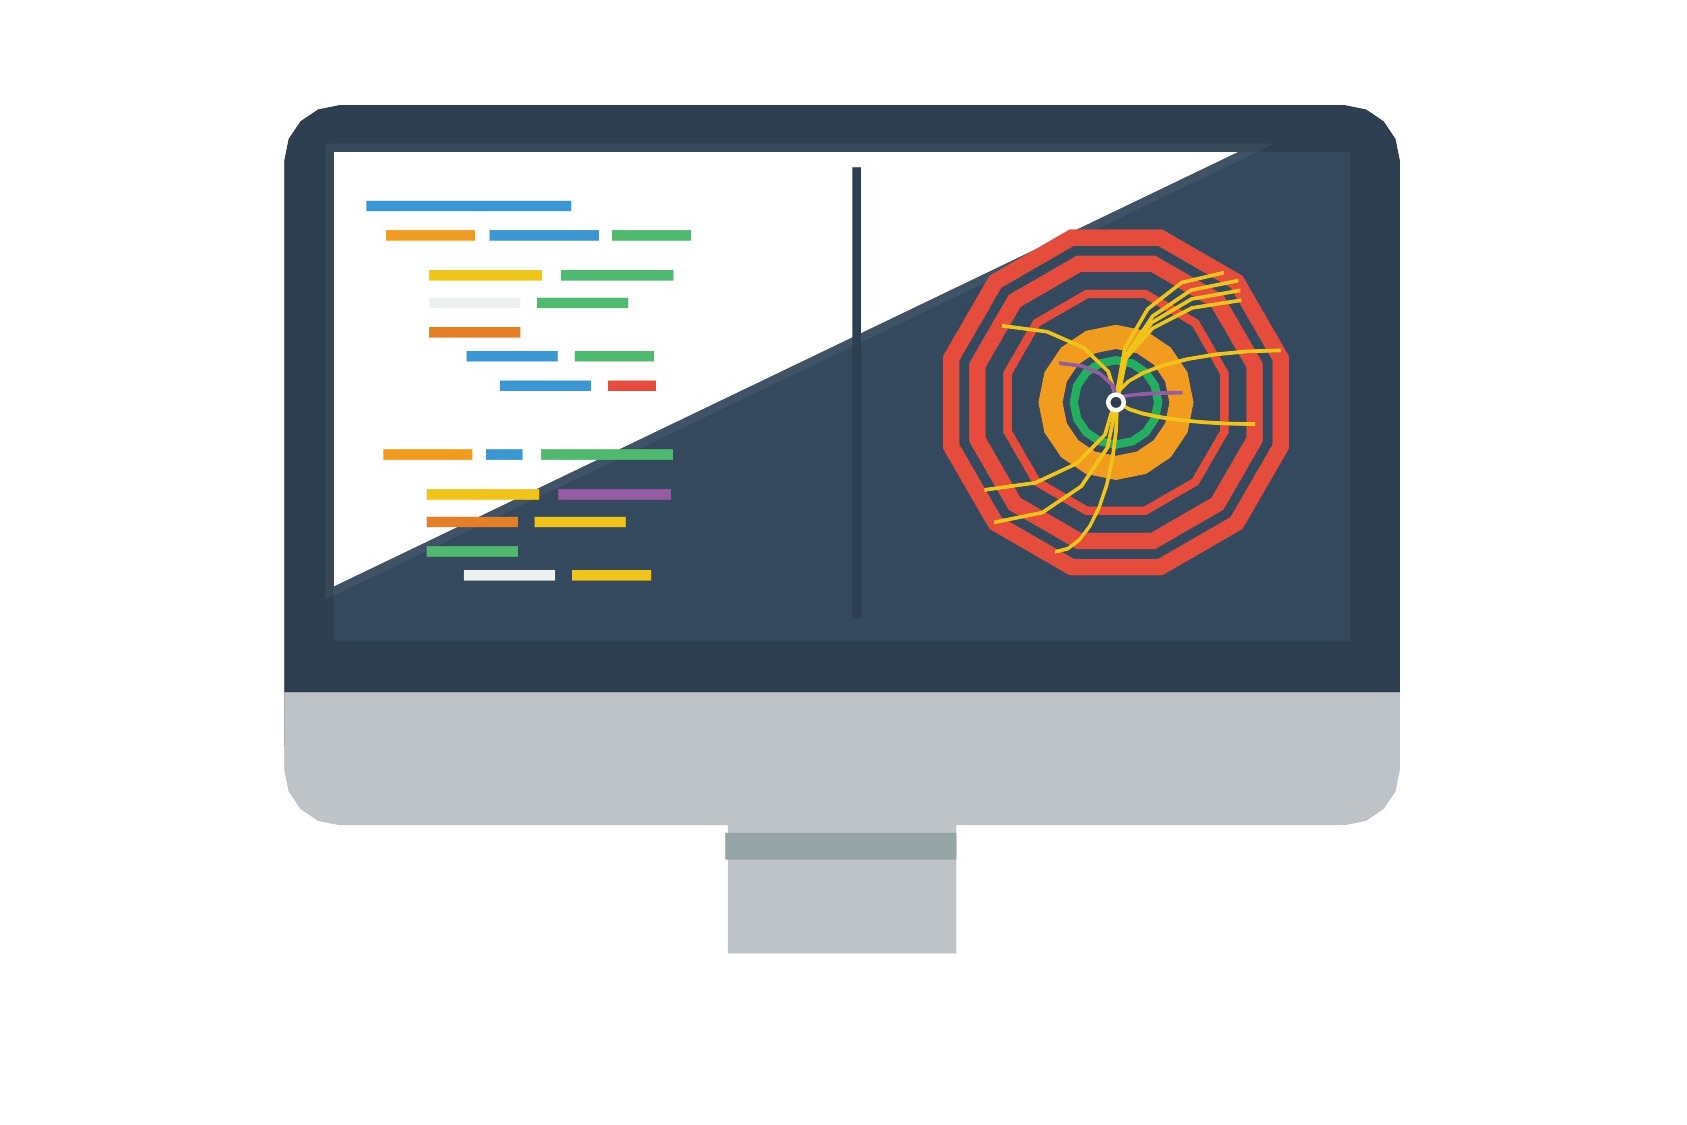
\includegraphics[width=0.9\textwidth]{images/better-software.jpg}
\end{figure}
\end{textblock}

\begin{textblock}{22.5}(44,77)
\textcolor{mybluelabel}{\bf Training} \\
Provide training for students in all of our core research topics.
\end{textblock}

\begin{textblock}{12.5}(67.5,77)
\begin{figure}[tbph]
\centering

\includegraphics[width=0.8\textwidth]{images/training.jpg}
\end{figure}
\end{textblock}


%\begin{textblock}{38.0}(4,25)
%\begin{block}{DIANA/HEP Goals}
%There are three interrelated areas of activity:
%\begin{itemize}
%\item \textbf{Performance:}
%we will greatly increase parallelism and eliminate CPU- and IO-bottlenecks to achieve higher processing rates necessary to efficiently
%and expeditiously analyze large volumes of data.
%We will address some key design and implementation
%issues from the early days of ROOT which impact
%not only performance, but also the manageability of the software.
%%The community libraries involved will include ROOT IO (RIO), RooFit
%and RooStats.
%
%\item \textbf{Interoperability:}
%we will reposition these key libraries to better interoperate with
%the larger scientific software ecosystem, transitioning the field
%to a more sustainable path where {\em new ideas
%and software developed elsewhere can be more easily used in particle physics}
%and our best products can be evaluated by other fields.
%We will create modular versions of the libraries that work
%both within the traditional ROOT framework as well as
%within other frameworks such as Hadoop MapReduce, Apache Spark,
%Mathematica, Python and R.
%
%\item \textbf{Collaborative Analysis:}
%we will provide new tools that build on the concept and emerging practices
%in particle physics that data analysis is a collaborative activity, involving
%many individuals working within a given experiment, working in different
%experiments and even between the experimental and theory communities.
%This will involve directly integrating into the analysis tool suite the
%ability to capture elements of analysis workflows needed to satisfy
%best practices in data preservation, analysis archival, reproducibility,
%and open access.
%\end{itemize}
%\end{block}
%\end{textblock}



\begin{textblock}{38.0}(44,25.0)
\begin{block}{The HEP Analysis Software Ecosystem}
ROOT (\url{https://root.cern.ch}) is
the {\em de-facto} home for most community analysis
software developed in particle physics and related fields. Begun at CERN in 1995,
it provides a sophisticated data format and serialization technology
%(used, as an example, for 200 PB of LHC Run 1 data)
as well as key software tools for
data modeling, likelihood fitting, statistics and
multivariate data analysis. It also has a broader range of
functionalities, not strictly tied to the data-intensive aspects
of our science, including interactive C++ analysis, histogramming,
graphics (2D and 3D), math libraries (matrix algebra), image manipulation,
and tools for distributed computing. Despite many pioneering and
innovative features, the components are seen as too coupled,
and limited by design decisions taken 20 years ago.
Given the challenges from technology evolution and analysis complexity,
we are at a point in the software lifecycle where large changes are needed,
much as ROOT replaced an earlier generation of
FORTRAN-based tools (PAW, HBOOK).
%ROOT is, however, the starting
%point for any plan to enable the our community to
%exploit exabyte-scale data sets.
DIANA/HEP is building on and improving these
community libraries, moving other existing software elements into
community libraries, and developing additional new tools.
\end{block}
\end{textblock}



%\begin{textblock}{38.0}(44,52)
%\begin{textblock}{56.0}(4,90)
\begin{textblock}{38.0}(4,85.5)
\begin{block}{Project Team}
\begin{itemize}
\item Peter Elmer (Lead PI) - {\it Princeton Univ., Dept. of Physics}
\item Brian P. Bockelman (PI) - {\it Univ. of Nebraska-Lincoln, Dept. of Computer Science and Engineering}
\item Kyle Cranmer (PI) - {\it New York Univ., Dept. of Physics \& Center for Data Science}
\item Michael D. Sokoloff (PI) - {\it Univ. of Cincinnati, Dept. of Physics}
\item Jinyang Li (Senior Personnel) - {\it New York Univ., Computer Science Dept.}
\item David Lange - {\it Princeton Univ., Dept. of Physics} (From Jan. 2016)
\item Gilles Louppe - {\it New York Univ., Dept. of Physics \& Center for Data Science} (From Oct. 2015)
\item James Pivarski - {\it Princeton Univ., Dept. of Physics} (From Jan. 2016)
\item Eduardo Rodrigues - {\it Univ. of Cincinnati, Dept. of Physics} (From Feb. 2016)
\item Zhe Zhang - {\it Univ. of Nebraska-Lincoln, Dept. of Computer Science and Engineering} (Ph.D.\ Student)
\item Chien-Chin Huang - {\it New York Univ., Computer Science Dept.} (Ph.D.\ Student) 
\end{itemize}
\end{block}
\end{textblock}

%\begin{textblock}{38.0}(4,70)
%\begin{block}{CERN}
%\begin{center}
%\begin{figure}[tbph]
%\centering
%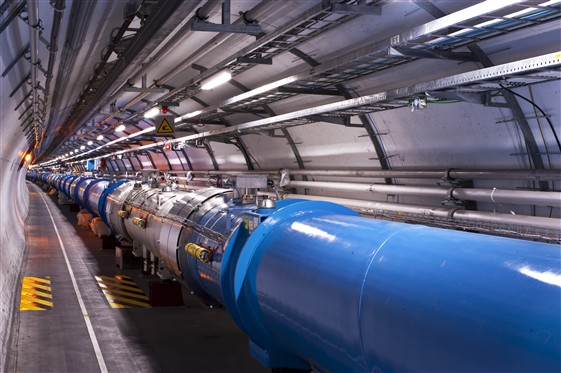
\includegraphics[width=1.0\textwidth]{images/0910152_02-A5-at-72-dpi.jpg}
%\end{figure}
%{\small 2009-2016 CERN (License: CC-BY-SA-4.0)}
%\end{center}
%\end{block}
%\end{textblock}


\begin{textblock}{38.0}(44,85.5)
\begin{block}{Advisory Board}
\begin{itemize}
\item Amber Boehnlein - {\it CIO, Thomas Jefferson National Accelerator Facility}
\item Katherine Copic - {\it Director of Growth, Insight Data Science}
\item Jacob VanderPlas - {\it Director of Research, Physical Sciences, eScience Institute, Univ. of Washington}
\item Fernando Perez - {\it Staff Scientist, Data Science and Technology Division, Lawrence Berkeley National Laboratory; Associate Researcher, Berkeley Institute for Data Science, UC Berkeley.}
\item Attanagoda Santha - {\it Architect, Fannie Mae}
\end{itemize}
\end{block}
\end{textblock}


%\begin{textblock}{78.0}(4,111)
%\begin{block}{Acknowledgement}
%This project is supported by National Science Foundation grants ACI-1450310, ACI-1450319, ACI-1450323, and ACI-1450377. Any opinions, findings, conclusions or recommendations expressed in this material are those of the developers and do not necessarily reflect the views of the National Science Foundation.
%\end{block}
%\end{textblock}

\begin{textblock}{38.0}(44,102)
\begin{block}{Acknowledgement}
This project is supported by National Science Foundation grants ACI-1450310, ACI-1450319, ACI-1450323, and ACI-1450377. Any opinions, findings, conclusions or recommendations expressed in this material are those of the developers and do not necessarily reflect the views of the National Science Foundation.
\end{block}
\end{textblock}




\end{frame}
\end{document}
